% Options for packages loaded elsewhere
\PassOptionsToPackage{unicode}{hyperref}
\PassOptionsToPackage{hyphens}{url}
%
\documentclass[
]{article}
\usepackage{amsmath,amssymb}
\usepackage{lmodern}
\usepackage{ifxetex,ifluatex}
\ifnum 0\ifxetex 1\fi\ifluatex 1\fi=0 % if pdftex
  \usepackage[T1]{fontenc}
  \usepackage[utf8]{inputenc}
  \usepackage{textcomp} % provide euro and other symbols
\else % if luatex or xetex
  \usepackage{unicode-math}
  \defaultfontfeatures{Scale=MatchLowercase}
  \defaultfontfeatures[\rmfamily]{Ligatures=TeX,Scale=1}
\fi
% Use upquote if available, for straight quotes in verbatim environments
\IfFileExists{upquote.sty}{\usepackage{upquote}}{}
\IfFileExists{microtype.sty}{% use microtype if available
  \usepackage[]{microtype}
  \UseMicrotypeSet[protrusion]{basicmath} % disable protrusion for tt fonts
}{}
\makeatletter
\@ifundefined{KOMAClassName}{% if non-KOMA class
  \IfFileExists{parskip.sty}{%
    \usepackage{parskip}
  }{% else
    \setlength{\parindent}{0pt}
    \setlength{\parskip}{6pt plus 2pt minus 1pt}}
}{% if KOMA class
  \KOMAoptions{parskip=half}}
\makeatother
\usepackage{xcolor}
\IfFileExists{xurl.sty}{\usepackage{xurl}}{} % add URL line breaks if available
\IfFileExists{bookmark.sty}{\usepackage{bookmark}}{\usepackage{hyperref}}
\hypersetup{
  pdftitle={ACME Case Study},
  pdfauthor={Team 14},
  hidelinks,
  pdfcreator={LaTeX via pandoc}}
\urlstyle{same} % disable monospaced font for URLs
\usepackage[margin=1in]{geometry}
\usepackage{color}
\usepackage{fancyvrb}
\newcommand{\VerbBar}{|}
\newcommand{\VERB}{\Verb[commandchars=\\\{\}]}
\DefineVerbatimEnvironment{Highlighting}{Verbatim}{commandchars=\\\{\}}
% Add ',fontsize=\small' for more characters per line
\usepackage{framed}
\definecolor{shadecolor}{RGB}{248,248,248}
\newenvironment{Shaded}{\begin{snugshade}}{\end{snugshade}}
\newcommand{\AlertTok}[1]{\textcolor[rgb]{0.94,0.16,0.16}{#1}}
\newcommand{\AnnotationTok}[1]{\textcolor[rgb]{0.56,0.35,0.01}{\textbf{\textit{#1}}}}
\newcommand{\AttributeTok}[1]{\textcolor[rgb]{0.77,0.63,0.00}{#1}}
\newcommand{\BaseNTok}[1]{\textcolor[rgb]{0.00,0.00,0.81}{#1}}
\newcommand{\BuiltInTok}[1]{#1}
\newcommand{\CharTok}[1]{\textcolor[rgb]{0.31,0.60,0.02}{#1}}
\newcommand{\CommentTok}[1]{\textcolor[rgb]{0.56,0.35,0.01}{\textit{#1}}}
\newcommand{\CommentVarTok}[1]{\textcolor[rgb]{0.56,0.35,0.01}{\textbf{\textit{#1}}}}
\newcommand{\ConstantTok}[1]{\textcolor[rgb]{0.00,0.00,0.00}{#1}}
\newcommand{\ControlFlowTok}[1]{\textcolor[rgb]{0.13,0.29,0.53}{\textbf{#1}}}
\newcommand{\DataTypeTok}[1]{\textcolor[rgb]{0.13,0.29,0.53}{#1}}
\newcommand{\DecValTok}[1]{\textcolor[rgb]{0.00,0.00,0.81}{#1}}
\newcommand{\DocumentationTok}[1]{\textcolor[rgb]{0.56,0.35,0.01}{\textbf{\textit{#1}}}}
\newcommand{\ErrorTok}[1]{\textcolor[rgb]{0.64,0.00,0.00}{\textbf{#1}}}
\newcommand{\ExtensionTok}[1]{#1}
\newcommand{\FloatTok}[1]{\textcolor[rgb]{0.00,0.00,0.81}{#1}}
\newcommand{\FunctionTok}[1]{\textcolor[rgb]{0.00,0.00,0.00}{#1}}
\newcommand{\ImportTok}[1]{#1}
\newcommand{\InformationTok}[1]{\textcolor[rgb]{0.56,0.35,0.01}{\textbf{\textit{#1}}}}
\newcommand{\KeywordTok}[1]{\textcolor[rgb]{0.13,0.29,0.53}{\textbf{#1}}}
\newcommand{\NormalTok}[1]{#1}
\newcommand{\OperatorTok}[1]{\textcolor[rgb]{0.81,0.36,0.00}{\textbf{#1}}}
\newcommand{\OtherTok}[1]{\textcolor[rgb]{0.56,0.35,0.01}{#1}}
\newcommand{\PreprocessorTok}[1]{\textcolor[rgb]{0.56,0.35,0.01}{\textit{#1}}}
\newcommand{\RegionMarkerTok}[1]{#1}
\newcommand{\SpecialCharTok}[1]{\textcolor[rgb]{0.00,0.00,0.00}{#1}}
\newcommand{\SpecialStringTok}[1]{\textcolor[rgb]{0.31,0.60,0.02}{#1}}
\newcommand{\StringTok}[1]{\textcolor[rgb]{0.31,0.60,0.02}{#1}}
\newcommand{\VariableTok}[1]{\textcolor[rgb]{0.00,0.00,0.00}{#1}}
\newcommand{\VerbatimStringTok}[1]{\textcolor[rgb]{0.31,0.60,0.02}{#1}}
\newcommand{\WarningTok}[1]{\textcolor[rgb]{0.56,0.35,0.01}{\textbf{\textit{#1}}}}
\usepackage{graphicx}
\makeatletter
\def\maxwidth{\ifdim\Gin@nat@width>\linewidth\linewidth\else\Gin@nat@width\fi}
\def\maxheight{\ifdim\Gin@nat@height>\textheight\textheight\else\Gin@nat@height\fi}
\makeatother
% Scale images if necessary, so that they will not overflow the page
% margins by default, and it is still possible to overwrite the defaults
% using explicit options in \includegraphics[width, height, ...]{}
\setkeys{Gin}{width=\maxwidth,height=\maxheight,keepaspectratio}
% Set default figure placement to htbp
\makeatletter
\def\fps@figure{htbp}
\makeatother
\setlength{\emergencystretch}{3em} % prevent overfull lines
\providecommand{\tightlist}{%
  \setlength{\itemsep}{0pt}\setlength{\parskip}{0pt}}
\setcounter{secnumdepth}{-\maxdimen} % remove section numbering
\ifluatex
  \usepackage{selnolig}  % disable illegal ligatures
\fi

\title{ACME Case Study}
\author{Team 14}
\date{4 6 2021}

\begin{document}
\maketitle

\hypertarget{introduction}{%
\section{Introduction}\label{introduction}}

\hypertarget{process-analytics}{%
\section{Process analytics}\label{process-analytics}}

\hypertarget{information-gathering}{%
\subsection{Information gathering}\label{information-gathering}}

Datensatz lesen und generellen Überblick verschaffen.

Zusammenfassung ausgeben

\begin{Shaded}
\begin{Highlighting}[]
\FunctionTok{summary}\NormalTok{(event\_log)}
\end{Highlighting}
\end{Shaded}

\begin{verbatim}
##    CASE_ID            ACTIVITY           TIMESTAMP                  
##  Length:178078      Length:178078      Min.   :2013-05-22 10:39:39  
##  Class :character   Class :character   1st Qu.:2018-06-11 09:41:52  
##  Mode  :character   Mode  :character   Median :2018-10-31 10:17:36  
##                                        Mean   :2018-10-16 14:14:51  
##                                        3rd Qu.:2019-02-23 10:12:57  
##                                        Max.   :2019-06-28 08:39:30  
##  REPAIR_IN_TIME_5D  DEVICETYPE        SERVICEPOINT      
##  Min.   :0.000     Length:178078      Length:178078     
##  1st Qu.:0.000     Class :character   Class :character  
##  Median :0.000     Mode  :character   Mode  :character  
##  Mean   :0.326                                          
##  3rd Qu.:1.000                                          
##  Max.   :1.000
\end{verbatim}

Ersten 10 Datensätzen ausgeben

\begin{Shaded}
\begin{Highlighting}[]
\FunctionTok{head}\NormalTok{(event\_log, }\AttributeTok{n=}\DecValTok{10}\NormalTok{)}
\end{Highlighting}
\end{Shaded}

\begin{verbatim}
## # A tibble: 10 x 6
##    CASE_ID ACTIVITY TIMESTAMP           REPAIR_IN_TIME_~ DEVICETYPE SERVICEPOINT
##    <chr>   <chr>    <dttm>                         <dbl> <chr>      <chr>       
##  1 Case10  Creation 2018-01-02 13:39:47                0 AB52       E           
##  2 Case10  Letter   2018-01-05 00:00:00                0 AB52       E           
##  3 Case10  DeviceR~ 2018-01-05 16:45:34                0 AB52       E           
##  4 Case10  StockEn~ 2018-01-17 00:00:00                0 AB52       E           
##  5 Case10  InDeliv~ 2018-01-17 00:00:00                0 AB52       E           
##  6 Case10  NoteWor~ 2018-01-17 07:37:19                0 AB52       E           
##  7 Case10  Complet~ 2018-01-17 09:34:32                0 AB52       E           
##  8 Case100 Creation 2018-01-02 15:43:48                0 AB41       E           
##  9 Case100 NoteHot~ 2018-01-02 15:44:41                0 AB41       E           
## 10 Case100 Letter   2018-01-08 00:00:00                0 AB41       E
\end{verbatim}

Wertebereich für interessante Spalten ausgeben

\begin{Shaded}
\begin{Highlighting}[]
\FunctionTok{unique}\NormalTok{(event\_log}\SpecialCharTok{$}\NormalTok{ACTIVITY)}
\end{Highlighting}
\end{Shaded}

\begin{verbatim}
##  [1] "Creation"       "Letter"         "DeviceReceived" "StockEntry"    
##  [5] "InDelivery"     "NoteWorkshop"   "Completed"      "NoteHotline"   
##  [9] "StatusRequest"  "Transmission"   "Approved"       "FreeticketCust"
## [13] "FreeticketComp"
\end{verbatim}

\begin{Shaded}
\begin{Highlighting}[]
\FunctionTok{unique}\NormalTok{(event\_log}\SpecialCharTok{$}\NormalTok{DEVICETYPE)}
\end{Highlighting}
\end{Shaded}

\begin{verbatim}
##  [1] "AB52" "AB41" "AB47" "AB22" "AB49" "AB62" "AB29" "AB63" "AB20" "AB53"
## [11] "AB50" "AB44" "AB45" "AB36" "AB61" "AB16" "AB34" "AB25" "AB40" "AB8" 
## [21] "AC68" "AB38" "AB65" "AB60" "AB31" "AB27" "AB10" "AB19" "AB59" "AB21"
## [31] "AB56" "AB26" "AB55" "AB9"  "AB58" "AB39" "AB14" "AB43" "AB24" "AO7" 
## [41] "AB57" "AB23" "AB28" "AB64" "AB32" "AB15" "AB30" "AF3"  "AB33" "AG5" 
## [51] "AB12" "AB51" "AB54" "AB18" "AB17" "AB35" "AB46" "AB37" "AB48" NA    
## [61] "AB42" "AG4"  "AB66" "AB67" "AB13"
\end{verbatim}

\begin{Shaded}
\begin{Highlighting}[]
\FunctionTok{unique}\NormalTok{(event\_log}\SpecialCharTok{$}\NormalTok{SERVICEPOINT)}
\end{Highlighting}
\end{Shaded}

\begin{verbatim}
##  [1] "E" "G" "J" "L" NA  "C" "H" "I" "K" "D" "B" "A"
\end{verbatim}

\begin{Shaded}
\begin{Highlighting}[]
\FunctionTok{unique}\NormalTok{(event\_log}\SpecialCharTok{$}\NormalTok{REPAIR\_IN\_TIME\_5D)}
\end{Highlighting}
\end{Shaded}

\begin{verbatim}
## [1] 0 1
\end{verbatim}

\hypertarget{data-cleaning}{%
\subsection{Data cleaning}\label{data-cleaning}}

Datensätze ohne Angabe zu Servicepoint oder Gerät ausschließen.

\begin{Shaded}
\begin{Highlighting}[]
\NormalTok{clean\_events }\OtherTok{\textless{}{-}} \FunctionTok{na.omit}\NormalTok{(event\_log)}
\end{Highlighting}
\end{Shaded}

Datensatz aus unvollständigen Sätzen abspalten.

\begin{Shaded}
\begin{Highlighting}[]
\NormalTok{corrupted\_events }\OtherTok{\textless{}{-}} \FunctionTok{subset}\NormalTok{(event\_log,}\FunctionTok{is.na}\NormalTok{(DEVICETYPE) }\SpecialCharTok{|} \FunctionTok{is.na}\NormalTok{(SERVICEPOINT))}
\end{Highlighting}
\end{Shaded}

\hypertarget{data-analytics}{%
\subsection{Data analytics}\label{data-analytics}}

Wie viele verschiedene Bearbeitungsfälle gibt es?

\begin{Shaded}
\begin{Highlighting}[]
\FunctionTok{unique}\NormalTok{(clean\_events}\SpecialCharTok{$}\NormalTok{CASE\_ID) }\SpecialCharTok{\%\textgreater{}\%} \FunctionTok{length}\NormalTok{()}
\end{Highlighting}
\end{Shaded}

\begin{verbatim}
## [1] 21931
\end{verbatim}

Wie sind die Events auf die Servicepoints verteilt?

\begin{Shaded}
\begin{Highlighting}[]
\CommentTok{\# servicepoints}
\NormalTok{servicepoints }\OtherTok{\textless{}{-}} \FunctionTok{table}\NormalTok{(clean\_events}\SpecialCharTok{$}\NormalTok{SERVICEPOINT)}

\NormalTok{sp\_df }\OtherTok{=} \FunctionTok{as.data.frame}\NormalTok{(servicepoints) }\SpecialCharTok{\%\textgreater{}\%} \FunctionTok{rename}\NormalTok{(}\AttributeTok{Servicepoint =}\NormalTok{ Var1)}

\NormalTok{sp\_distro\_plot }\OtherTok{\textless{}{-}} \FunctionTok{ggplot}\NormalTok{(}\AttributeTok{data=}\NormalTok{sp\_df, }\FunctionTok{aes}\NormalTok{(}\AttributeTok{x =}\NormalTok{ Servicepoint, }\AttributeTok{y=}\NormalTok{ Freq, }\AttributeTok{label=}\NormalTok{ Freq)) }\SpecialCharTok{+}
  \FunctionTok{geom\_bar}\NormalTok{(}\AttributeTok{stat=}\StringTok{"identity"}\NormalTok{) }\SpecialCharTok{+}
  \FunctionTok{geom\_text}\NormalTok{(}\AttributeTok{size =} \DecValTok{3}\NormalTok{, }\AttributeTok{position =} \FunctionTok{position\_stack}\NormalTok{(}\AttributeTok{vjust =} \FloatTok{0.5}\NormalTok{))}

\NormalTok{sp\_distro\_plot}
\end{Highlighting}
\end{Shaded}

\includegraphics{wi_sem_team_14_files/figure-latex/sp-distro-1.pdf}
5-Tage-Reperatur-Quote nach Servicepoint

\begin{Shaded}
\begin{Highlighting}[]
\CommentTok{\# das reperaturzeit flag steht in jedem eintrag eines CASEs, uns langt aber ein }
\CommentTok{\# Eintrag je CASE}
\NormalTok{distinct\_cases }\OtherTok{\textless{}{-}} \FunctionTok{distinct}\NormalTok{(clean\_events, CASE\_ID, }\AttributeTok{.keep\_all =} \ConstantTok{TRUE}\NormalTok{)}

\CommentTok{\# nach Servicepoint gruppieren und die flags aufsummieren}
\NormalTok{by\_servicep }\OtherTok{\textless{}{-}} \FunctionTok{group\_by}\NormalTok{(distinct\_cases, SERVICEPOINT) }\SpecialCharTok{\%\textgreater{}\%}
  \FunctionTok{summarise}\NormalTok{(}\AttributeTok{fivedaysum =} \FunctionTok{sum}\NormalTok{(REPAIR\_IN\_TIME\_5D), }\AttributeTok{all =} \FunctionTok{n}\NormalTok{())}
\CommentTok{\# quote berechnen mit anzahl der "schnellen" CASEs}
\NormalTok{by\_servicep}\SpecialCharTok{$}\NormalTok{quota }\OtherTok{=}\NormalTok{ by\_servicep}\SpecialCharTok{$}\NormalTok{fivedaysum }\SpecialCharTok{/}\NormalTok{ by\_servicep}\SpecialCharTok{$}\NormalTok{all }\SpecialCharTok{*} \DecValTok{100}

\CommentTok{\# plot zeichnen}
\NormalTok{plot }\OtherTok{\textless{}{-}} \FunctionTok{ggplot}\NormalTok{(}\AttributeTok{data =}\NormalTok{ by\_servicep, }\FunctionTok{aes}\NormalTok{(}\AttributeTok{x=}\NormalTok{SERVICEPOINT, }\AttributeTok{y=}\NormalTok{quota, }\AttributeTok{label=}\NormalTok{all)) }\SpecialCharTok{+}
  \FunctionTok{geom\_bar}\NormalTok{(}\AttributeTok{stat=}\StringTok{"identity"}\NormalTok{) }\SpecialCharTok{+} \FunctionTok{ylab}\NormalTok{(}\StringTok{"}\SpecialCharTok{\textbackslash{}"}\StringTok{In time}\SpecialCharTok{\textbackslash{}"}\StringTok{ repair quota in \%"}\NormalTok{)}\SpecialCharTok{+}
  \FunctionTok{xlab}\NormalTok{(}\StringTok{"Servicepoint"}\NormalTok{) }\SpecialCharTok{+}
  \FunctionTok{geom\_text}\NormalTok{(}\AttributeTok{size =} \DecValTok{3}\NormalTok{, }\AttributeTok{position =} \FunctionTok{position\_stack}\NormalTok{(}\AttributeTok{vjust =} \FloatTok{0.5}\NormalTok{))}
\NormalTok{plot}
\end{Highlighting}
\end{Shaded}

\includegraphics{wi_sem_team_14_files/figure-latex/5-day-quota-1.pdf}
Clusteranalyse Anfälligkeit der Geräte

\begin{Shaded}
\begin{Highlighting}[]
\NormalTok{case\_total\_duration }\OtherTok{\textless{}{-}} \FunctionTok{group\_by}\NormalTok{(clean\_events, CASE\_ID) }\SpecialCharTok{\%\textgreater{}\%}
  \FunctionTok{group\_by}\NormalTok{(DEVICETYPE, }\AttributeTok{.add =} \ConstantTok{TRUE}\NormalTok{) }\SpecialCharTok{\%\textgreater{}\%}
  \FunctionTok{summarise}\NormalTok{(}\AttributeTok{timemax =} \FunctionTok{max}\NormalTok{(TIMESTAMP), }\AttributeTok{timemin =} \FunctionTok{min}\NormalTok{(TIMESTAMP), }\AttributeTok{duration =}\NormalTok{ timemax }\SpecialCharTok{{-}}\NormalTok{ timemin)}
\end{Highlighting}
\end{Shaded}

\begin{verbatim}
## `summarise()` has grouped output by 'CASE_ID'. You can override using the `.groups` argument.
\end{verbatim}

\begin{Shaded}
\begin{Highlighting}[]
\NormalTok{avg\_duration\_by\_device }\OtherTok{\textless{}{-}}\NormalTok{ case\_total\_duration }\SpecialCharTok{\%\textgreater{}\%}
  \FunctionTok{group\_by}\NormalTok{(DEVICETYPE) }\SpecialCharTok{\%\textgreater{}\%}
  \FunctionTok{summarize}\NormalTok{(}\AttributeTok{case\_count =} \FunctionTok{n}\NormalTok{(), }\AttributeTok{avg\_time =} \FunctionTok{mean}\NormalTok{(duration))}

\NormalTok{avg\_duration\_by\_device}\SpecialCharTok{$}\NormalTok{avg\_time }\OtherTok{\textless{}{-}} \FunctionTok{as.numeric}\NormalTok{(avg\_duration\_by\_device}\SpecialCharTok{$}\NormalTok{avg\_time, }\AttributeTok{units=}\StringTok{"days"}\NormalTok{)}

\FunctionTok{ggplot}\NormalTok{(avg\_duration\_by\_device, }\FunctionTok{aes}\NormalTok{(case\_count, avg\_time)) }\SpecialCharTok{+} \FunctionTok{geom\_point}\NormalTok{()}
\end{Highlighting}
\end{Shaded}

\includegraphics{wi_sem_team_14_files/figure-latex/cluster-1.pdf}

\begin{Shaded}
\begin{Highlighting}[]
\NormalTok{h.cluster }\OtherTok{\textless{}{-}}\NormalTok{ avg\_duration\_by\_device }\SpecialCharTok{\%\textgreater{}\%} \FunctionTok{dist}\NormalTok{(., }\AttributeTok{method =} \StringTok{"euclidean"}\NormalTok{) }\SpecialCharTok{\%\textgreater{}\%} \FunctionTok{hclust}\NormalTok{(., }\AttributeTok{method=}\StringTok{"ward.D"}\NormalTok{)}
\end{Highlighting}
\end{Shaded}

\begin{verbatim}
## Warning in dist(., method = "euclidean"): NAs durch Umwandlung erzeugt
\end{verbatim}

\begin{Shaded}
\begin{Highlighting}[]
\FunctionTok{plot}\NormalTok{(h.cluster)}
\end{Highlighting}
\end{Shaded}

\includegraphics{wi_sem_team_14_files/figure-latex/cluster-2.pdf}

\begin{Shaded}
\begin{Highlighting}[]
\NormalTok{p.cluster }\OtherTok{\textless{}{-}}\NormalTok{ avg\_duration\_by\_device }\SpecialCharTok{\%\textgreater{}\%} \FunctionTok{select}\NormalTok{(avg\_time, case\_count) }\SpecialCharTok{\%\textgreater{}\%} \FunctionTok{kmeans}\NormalTok{(., }\DecValTok{3}\NormalTok{)}
\NormalTok{p.cluster}\SpecialCharTok{$}\NormalTok{cluster }\OtherTok{\textless{}{-}} \FunctionTok{as.factor}\NormalTok{(p.cluster}\SpecialCharTok{$}\NormalTok{cluster)}

\FunctionTok{ggplot}\NormalTok{(avg\_duration\_by\_device, }\FunctionTok{aes}\NormalTok{(case\_count, avg\_time, }\AttributeTok{label =}\NormalTok{ DEVICETYPE)) }\SpecialCharTok{+} 
  \FunctionTok{scale\_fill\_discrete}\NormalTok{(}\AttributeTok{name =} \StringTok{"Cluster"}\NormalTok{) }\SpecialCharTok{+} 
  \FunctionTok{geom\_label}\NormalTok{(}\FunctionTok{aes}\NormalTok{(}\AttributeTok{fill =}\NormalTok{ p.cluster}\SpecialCharTok{$}\NormalTok{cluster), }\AttributeTok{colour =} \StringTok{"white"}\NormalTok{, }\AttributeTok{fontface =} \StringTok{"bold"}\NormalTok{, }\AttributeTok{size =} \DecValTok{2}\NormalTok{)}
\end{Highlighting}
\end{Shaded}

\includegraphics{wi_sem_team_14_files/figure-latex/cluster-3.pdf}

\hypertarget{celonis}{%
\subsection{Celonis}\label{celonis}}

``Happy Path'' + throughput time per month: optimal sequence of
activities takes an average of 24 days, all paths got 17 days average
duration throughput time was on its maximum in October 2018 (24 days)
and took 20 days in January, February and April, the second highest
duration cases before year 2018 were erased as in other analytics
because first cases documented were in 2013, but with throughput times
of 5 years (and missing entries?)
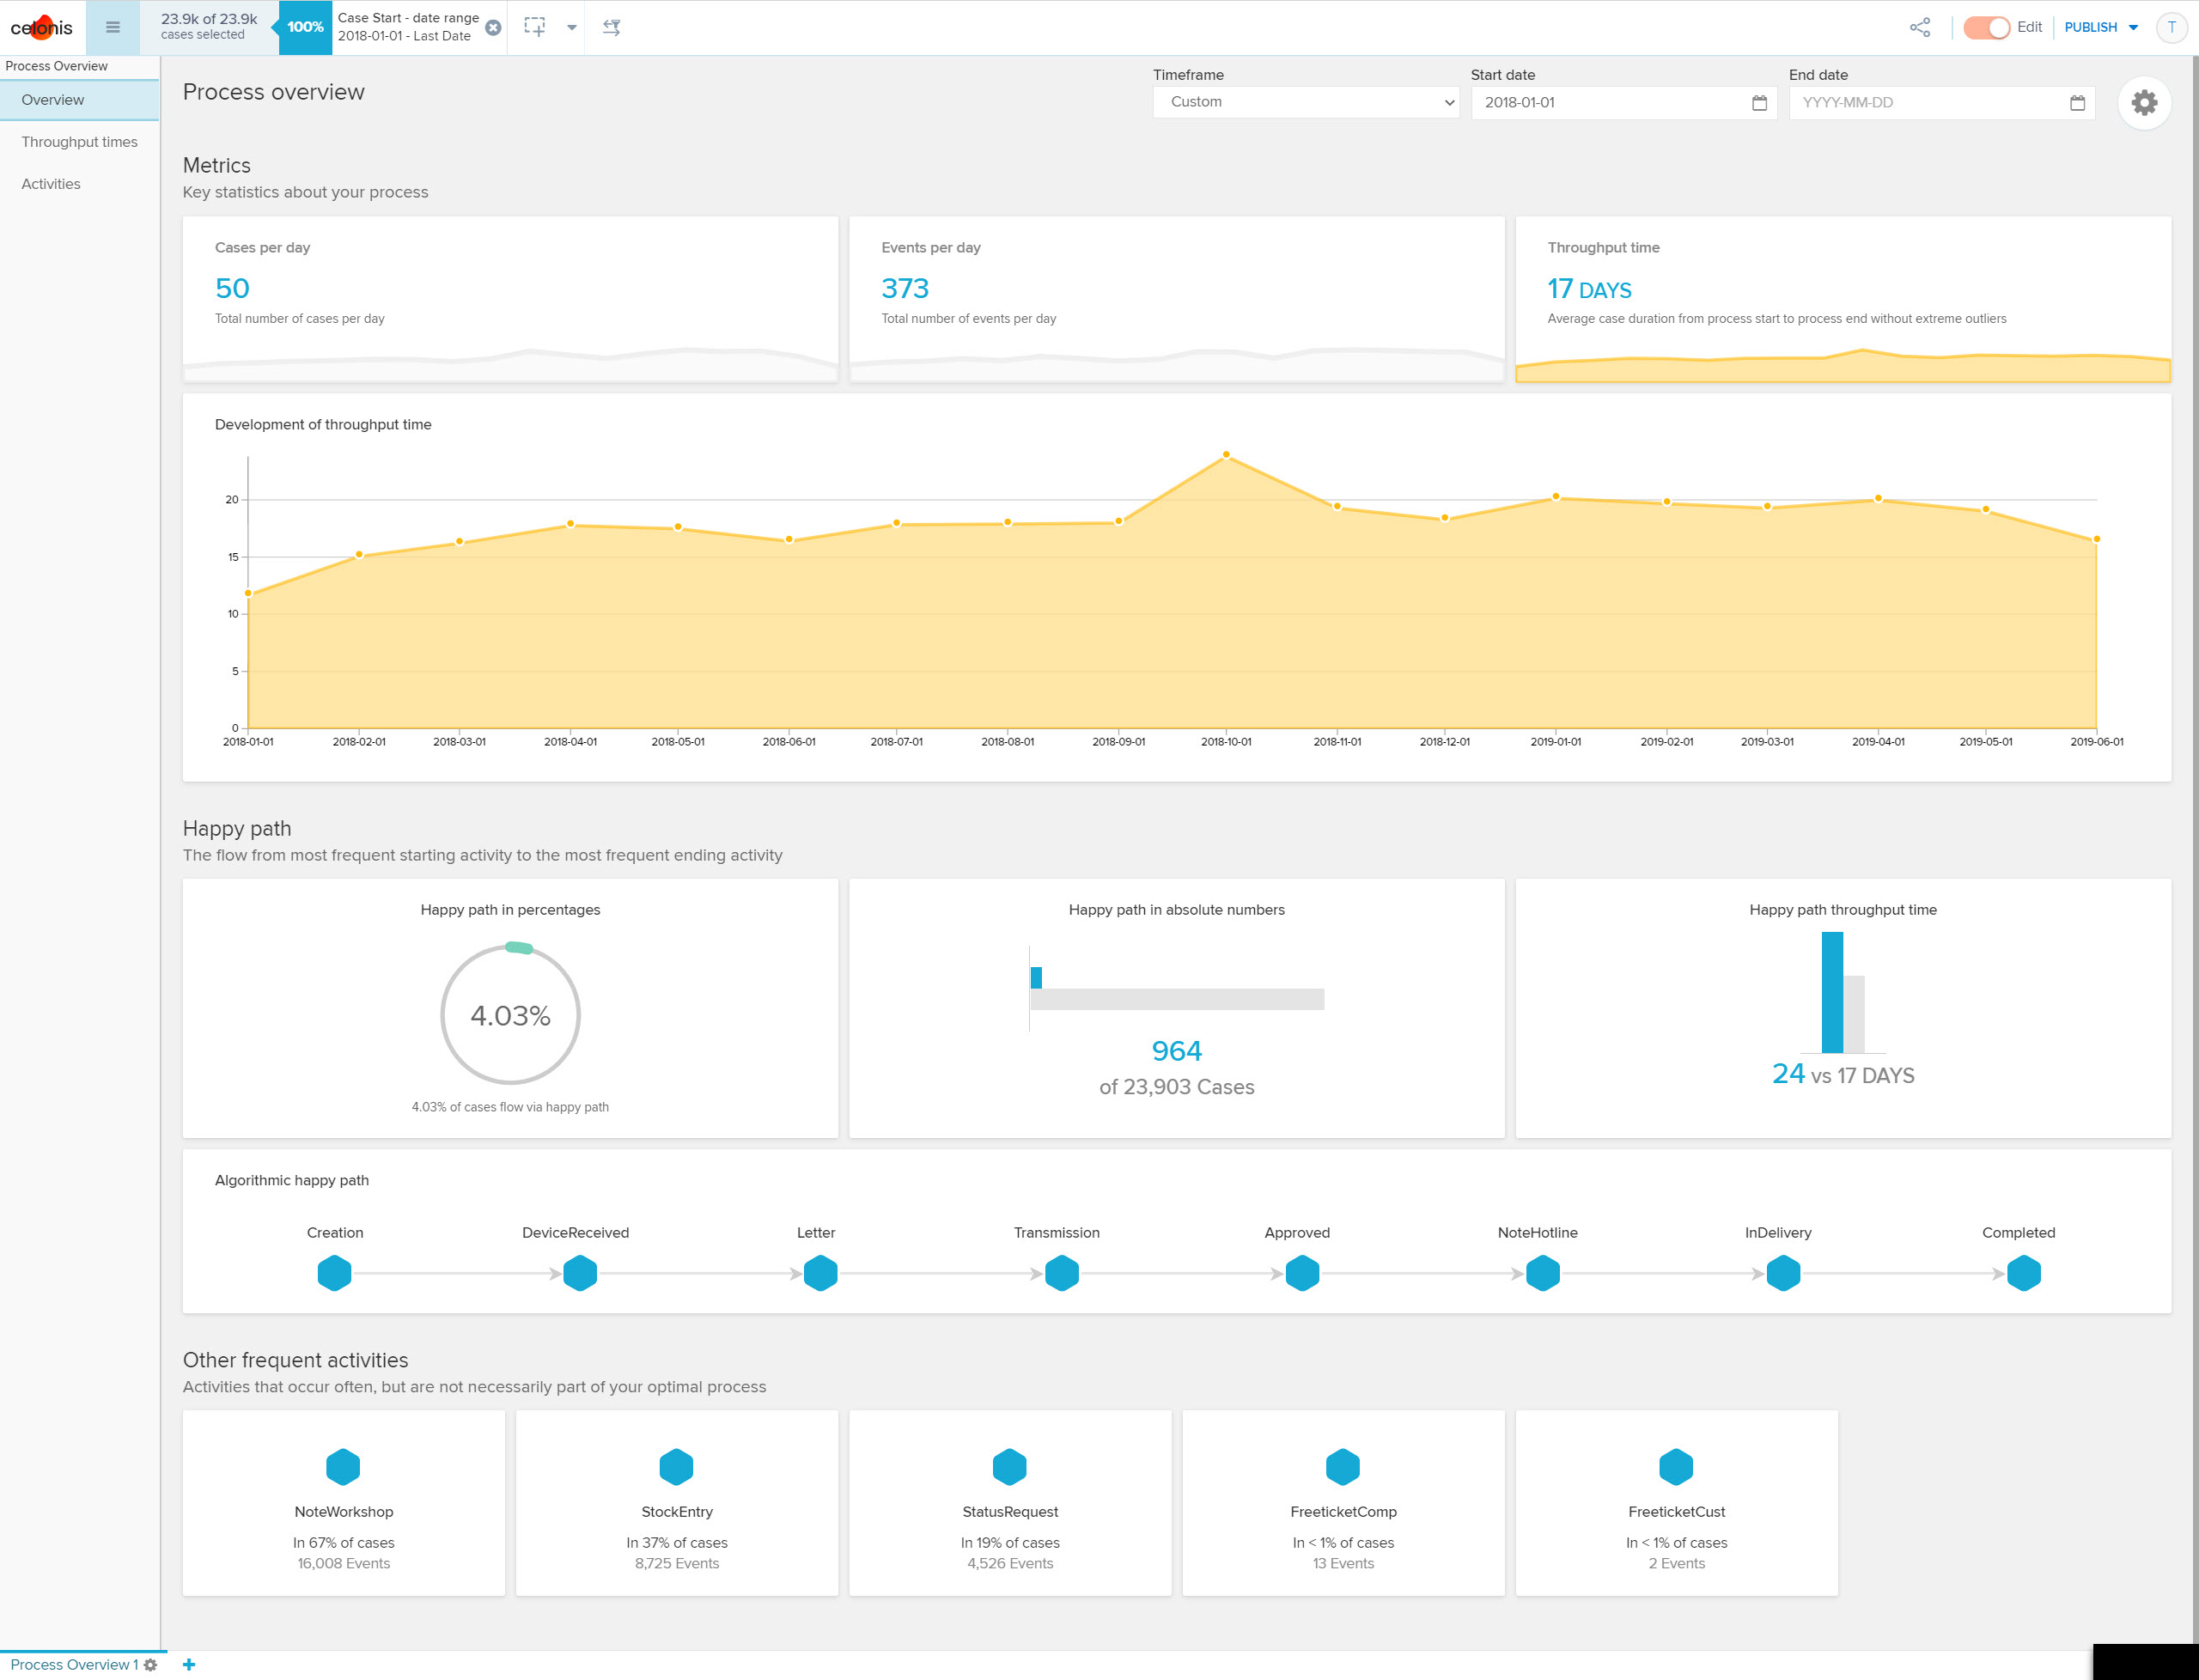
\includegraphics{https://github.com/CTM-development/WI_Seminar/blob/main/celonis_imgs/HappyPath+DurationPerMonth.jpg?raw=true}

``Happy Path'' + average case number per day in one month: case count
was highest in October 2018 (103 cases), February 2019 (107), March 2019
(102) and April 2019 (103) regarding the previous celonis analysis the
throughput time per month and the average of cases per day in one month
can be seen in relation to each other
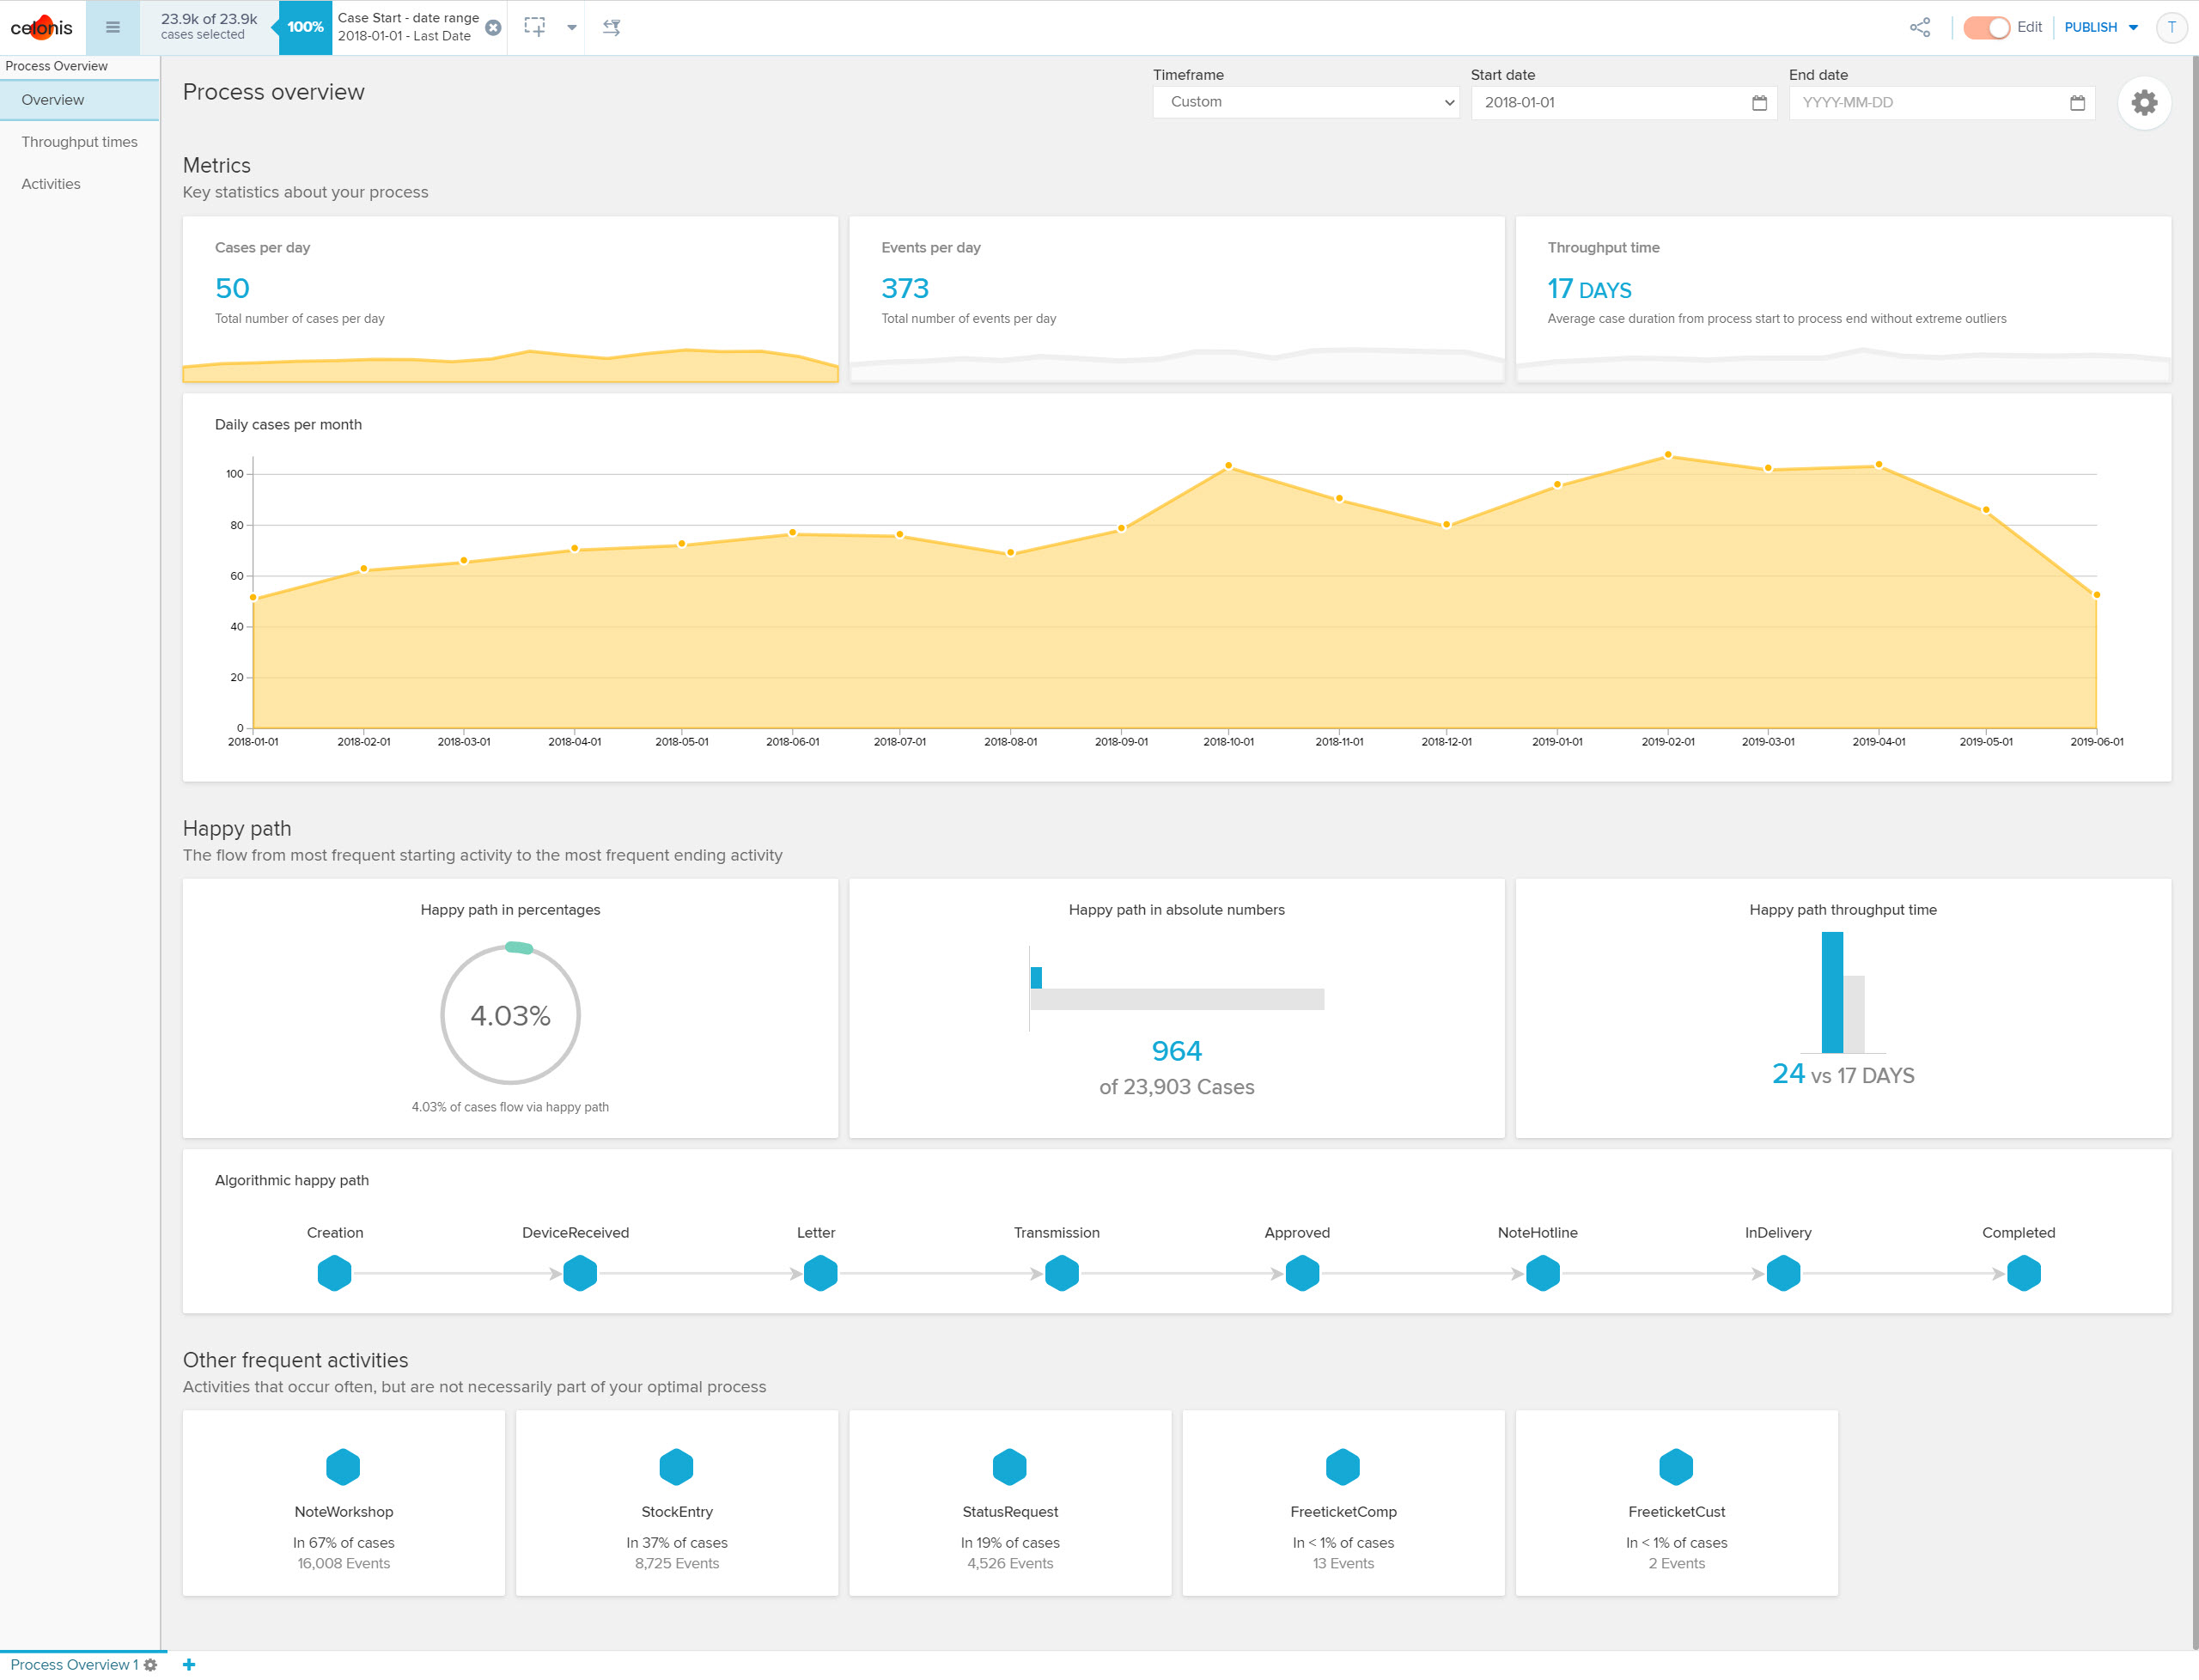
\includegraphics{https://github.com/CTM-development/WI_Seminar/blob/main/celonis_imgs/HappyPath+CasesPerDay.jpg?raw=true}

Bottlenecks:
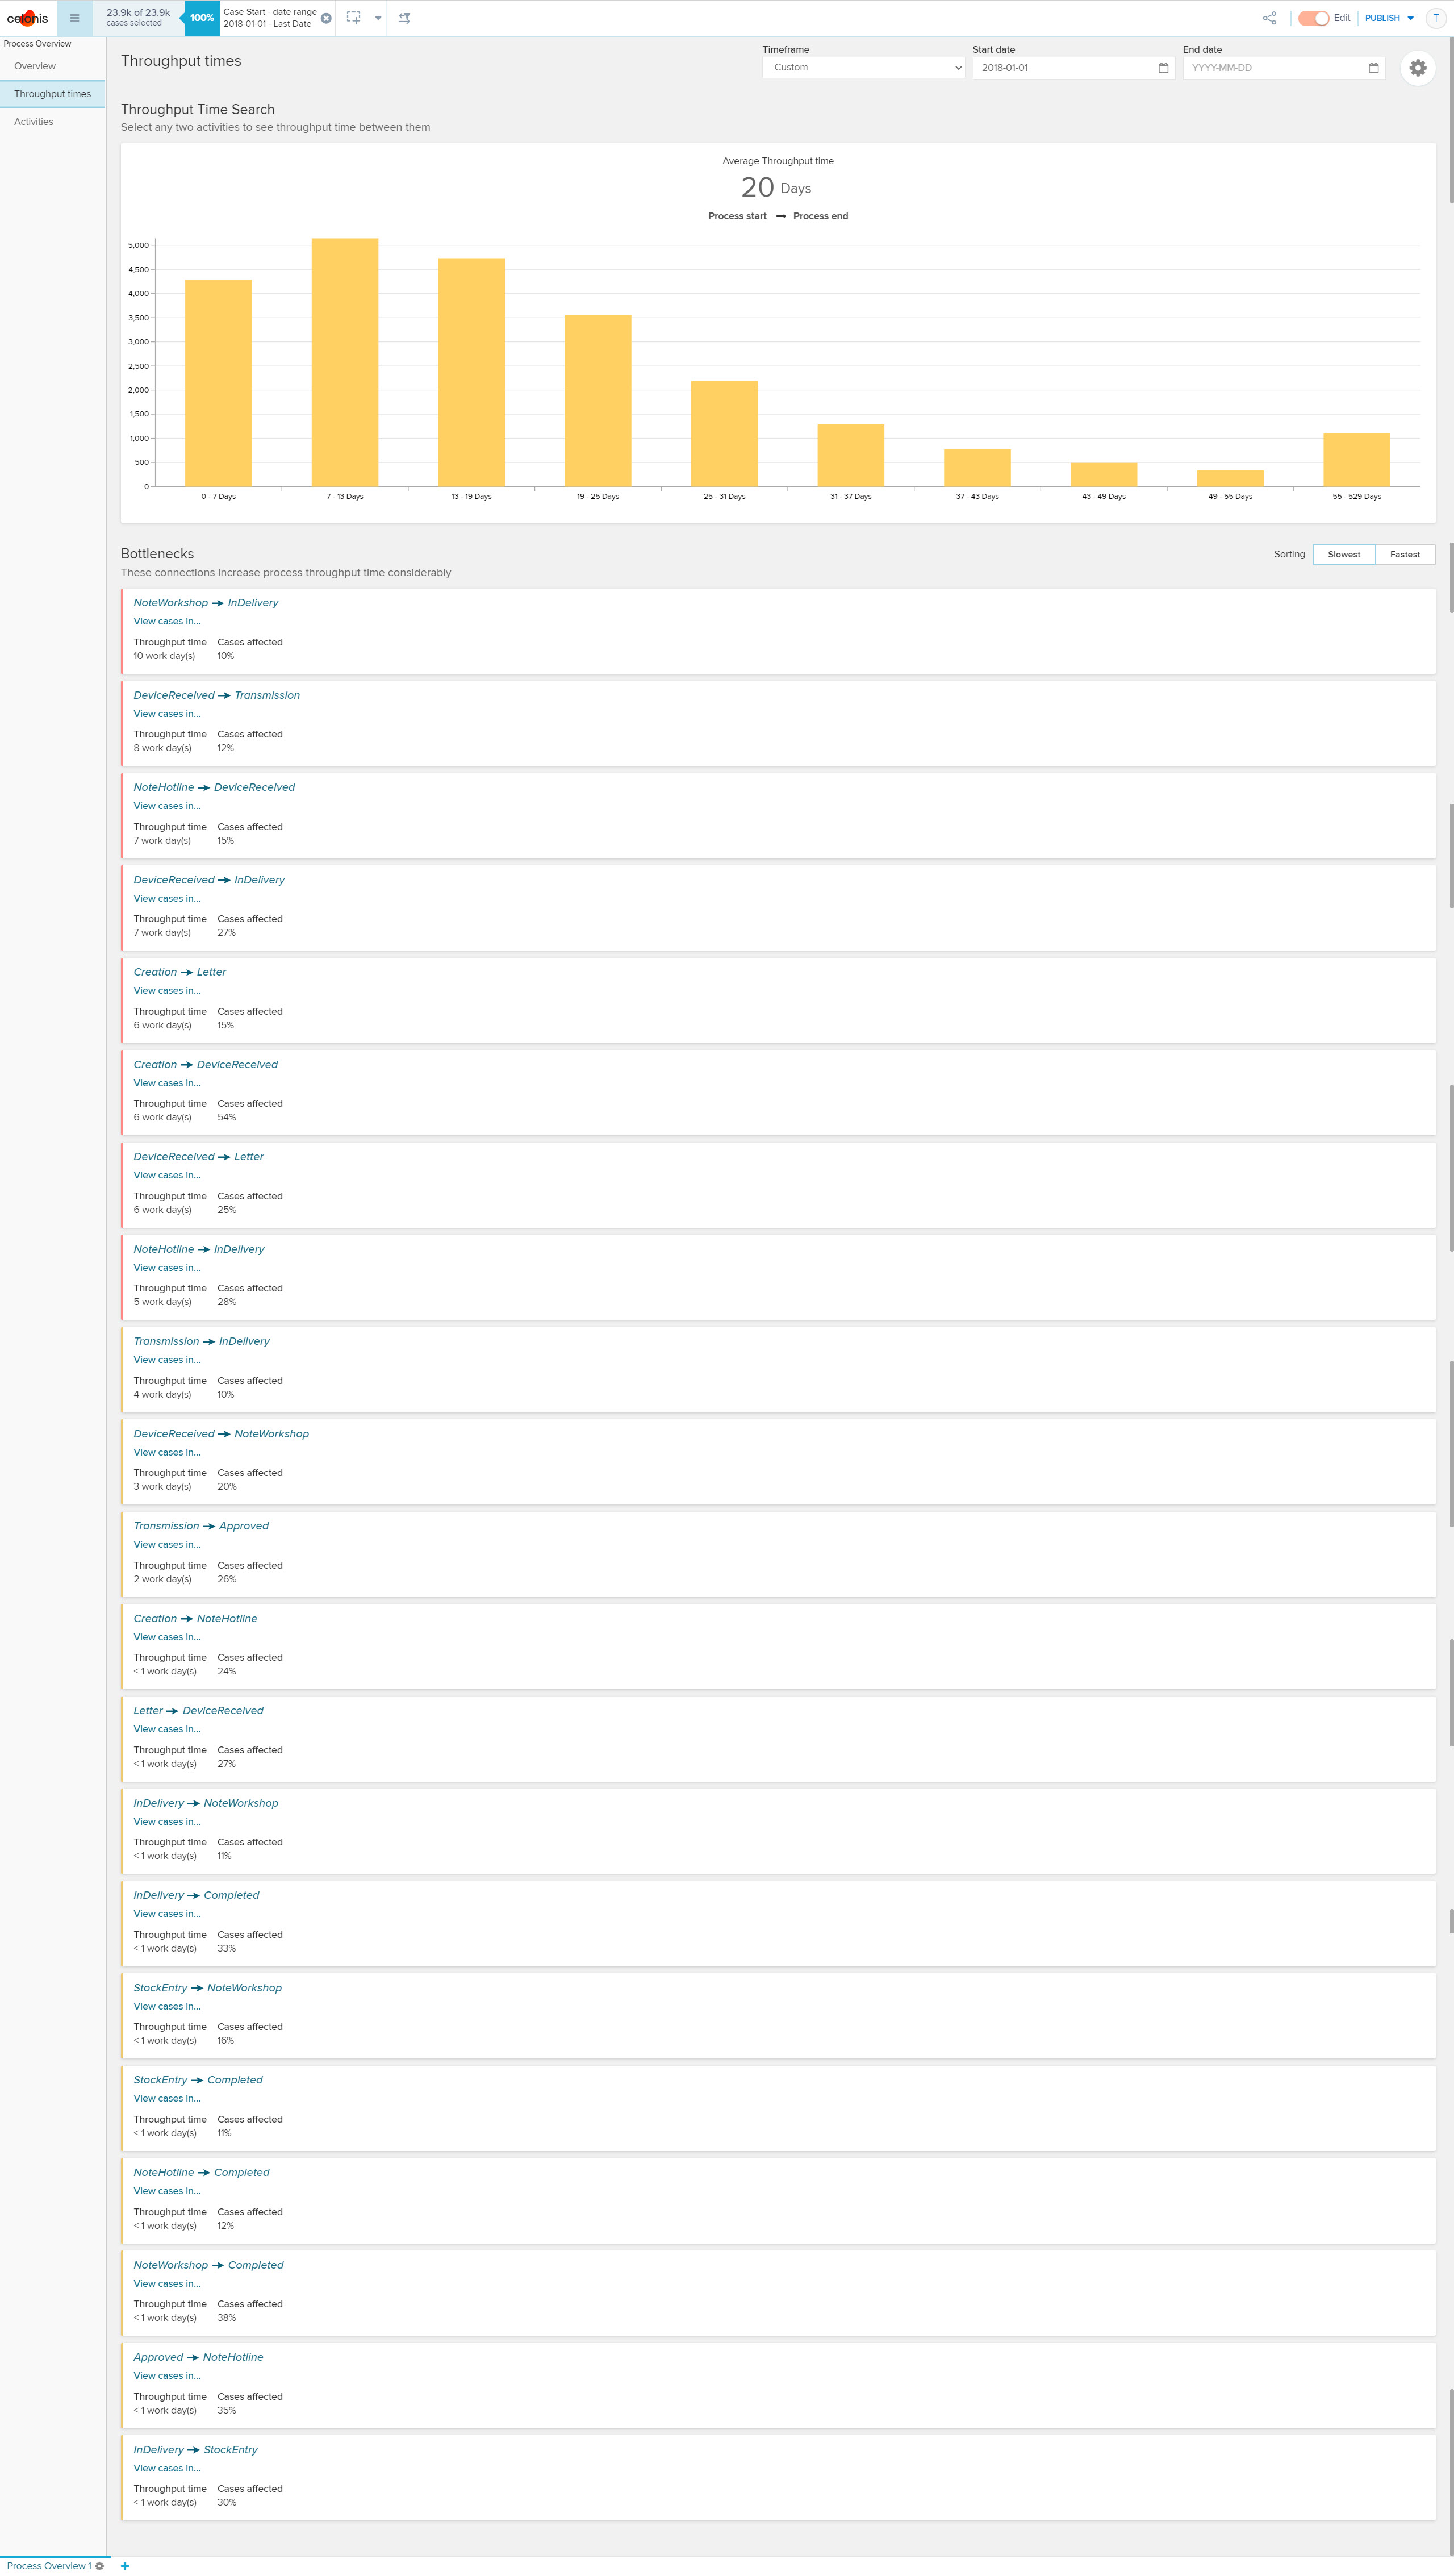
\includegraphics{https://github.com/CTM-development/WI_Seminar/blob/main/celonis_imgs/Bottlenecks.jpg?raw=true}

Path with shortest throughput time:
\includegraphics{https://github.com/CTM-development/WI_Seminar/blob/main/celonis_imgs/Path\%20with\%20shortest\%20Throughput\%20Time.PNG?raw=true}

Top 10 paths with the shortest throughput times: no improvements needed
conforms 0\% of all paths
\includegraphics{https://github.com/CTM-development/WI_Seminar/blob/main/Top\%2010\%20shortest\%20Throughput\%20Time.jpg?raw=true}

Top 10 paths with the longest throughput times: should be improved
\includegraphics{https://github.com/CTM-development/WI_Seminar/blob/main/Top\%2010\%20longest\%20Throughput\%20Time.jpg?raw=true}

Top 10 most common paths: conform to 21\% of all possible paths
\includegraphics{https://github.com/CTM-development/WI_Seminar/blob/main/Top10\%20Most\%20Common.jpg?raw=true}

\hypertarget{business-implications}{%
\section{Business implications}\label{business-implications}}

\hypertarget{optimizing-load-distribution}{%
\subsection{Optimizing load
distribution}\label{optimizing-load-distribution}}

Currently the distribution of the workload among the servicepoints is
suboptimal. The servicepoints E and L account for the majority of
events, while A - D barely logged anything. This leads us to the
assumption that most of the service cases are being processed by those
SPs. We expect that an equal distribution of the workload between all
available SPs would lead to an increase in repair speed and total
capacity.

\hypertarget{error-prone-devices}{%
\subsection{Error-prone devices}\label{error-prone-devices}}

Different devices have a different proneness to technical failure. The
underlying assumption is that those devices which are most likely to
fail, will be brought in for service the most often. Also the devices
differ in how long it takes on average to repair them. Using these two
factors, one can estimate how service and resource intensive these
devices are during their lifetime.

The cluster analysis shows which devices are the most resource intensive
ones by dividing them into three groups. The most error-prone device,
with over 3000 service cases in the observed timespan and an average
repair time of 27 days is the model AB52. We suggest removing this
device from the product portfolio, as frequent failure of the device has
a negative impact on customer satisfaction.

\hypertarget{improve-data-collection}{%
\subsection{Improve data collection}\label{improve-data-collection}}

In order to perform detailed analysis of the service process, more data
about the timing of activities is needed. Currently only the completion
time of an activity is logged. We recommend to also track the start time
of each activity. This way it's possible to make statements about the
real duration of the activity and possible idle-times. As of now, it's
impossible to say if an activity took a lot of time or if there was a
lot of idle-time before it started. Also there were some event logs
without information about the associated servicepoint. We recommend to
install mechanisms that prevent incomplete logs from being saved.

\end{document}
